\documentclass{report}
\usepackage[utf8]{inputenc}

\usepackage[italian]{babel}
\usepackage[italian]{cleveref}
\usepackage{graphicx}

\title{OOP-FARGOAL}
\author{
    Bulgarelli Marco, marco.bulgarelli@studio.unibo.it \and 
    Ravaioli Alessandro, alessandro.ravaioli@studio.unibo.it \and
    Tassinari Sabrina, sabrina.tassinari@studio.unibo.it \and
    Tramonti Daniele, daniele.tramonti@studio.unibo.it 
}
\date{15 febbraio 2025}

\begin{document}
\maketitle

\tableofcontents

\chapter{Analisi}

\section{Desctizione e requisiti}

Il software mira alla costruzione di un videogioco ispirato a “Sword of Fargoal”. 
%
Quest’ultimo è un “Dungeon Crawler Arcade”, ovvero basato sull’esplorazione di un labirinto a più piani, con lo scopo di riportare in superficie la Spada di Fargoal attraversando innumerevoli pericoli. 
%
La nostra versione cercherà di essere il più fedele possibile al gioco originale.

\subsection{Requisiti funzionali}
\begin{itemize}
    \item Il giocatore si muoverà all’interno di una grande stanza che corrisponde ad un piano del Dungeon. La generazione di ogni piano (e dei suoi contenuti) dovrà essere casuale.
    \item Il piano è caratterizzato dalla presenza di mostri. Questi possono apparire in luoghi specifici o in punti casuali, aumentando gradualmente con il passare del tempo, rendendo l’ambiente sempre più pericoloso.
    \item All’interno del piano saranno presenti due tipologie di oggetti di cui il giocatore potrà usufruire: dei bauli, che possono contenere degli oggetti magici o delle trappole, oppure delle sacche di monete.
    \item Il sistema di progresso del personaggio è legato all’accumulo di esperienza, che contribuisce all’aumentare del suo livello. Questa può essere ottenuta sia combattendo contro i mostri che offrendo donazioni in oro ai templi.
    \item In ogni piano sarà presente almeno un tempio, dove è possibile donare oro per salire di livello, rigenerare punti ferita e, ogni volta che sono state donate 2000 monete, di essere curati completamente. Inoltre, i templi garantiscono temporanea inattaccabilità ed una rigenerazione accelerata.
    \item Una volta recuperata la spada, è necessario riportarla in superficie, ritornando al primo piano e salendo le scale per uscire dal labirinto. La sfida sta nel fatto che, se il giocatore viene attaccato da un mostro, perde la spada, che ritornerà automaticamente nel piano in cui è stata trovata.
\end{itemize}

\subsection{Modello del dominio}

Il labirinto (\textit{dungeon}) è formato da più piani (\textit{Floor}). 
%
Per muoversi fra un piano e l’altro si utilizzeranno delle rampe di scale; in uno stesso piano saranno presenti più rampe per risalire o per scendere. 
%
Ogni volta che si entra in un nuovo piano, che sia antecedente o successivo, esso verrà generato casualmente. 
%
All’interno di ogni piano saranno presenti vari elementi (in \ref{Figura 1.1} si chiamano \textit{FloorElement}): alcuni hanno la caratteristica di essere interagibili (\textit{Interactable}), mentre gli altri elementi sono delle entità (\textit{Entity}), che si muovono all’interno del piano. 
%
I primi, che sono fissi nella mappa, sono l’insieme formato dalle ceste (che contengono oggetti magici), le scale (in \ref{Figura 1.1} \textit{Stairs}) e il tempio (in \ref{Figura 1.1} \textit{Temple}) , che è unico all’interno del piano. 
%
Le entità, invece, sono l’insieme dei mostri (in \ref{Figura 1.1} \textit{Monster}) e del giocatore (in \ref{Figura 1.1} \textit{Player}); entrambi si muovono liberamente all’interno del piano e possono entrare in combattimento l’uno con l’altro. 

\begin{figure}
    \centering
    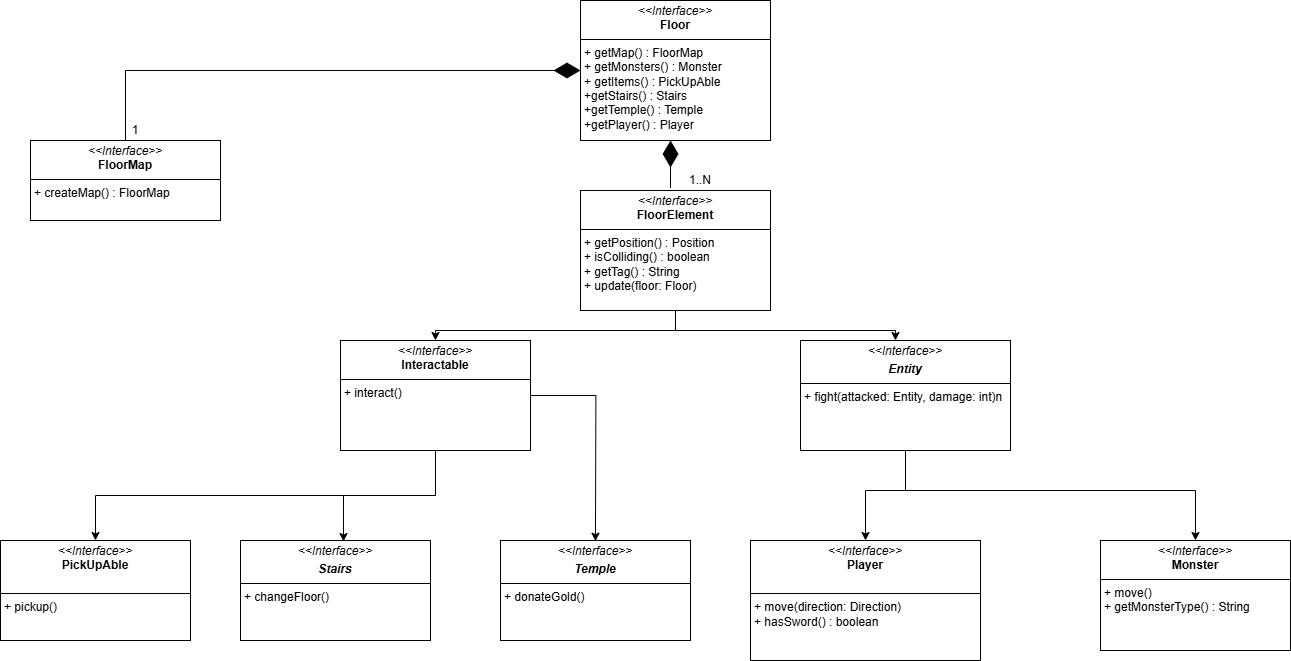
\includegraphics[width=12cm]{DiagrammaUMLGenerale.png}
    \caption{Schema UML dell'analisi del problema, con rappresentate le entità principali ed i rapporti fra di loro}
    \label{Figura 1.1}
\end{figure}

\chapter{Design}

\section{Architettura}

\section{Design dettagliato}

\subsection{Bulgarelli Marco}

\subsection{Ravaioli Alessandro}

\subsection{Tassinari Sabrina}

\subsection{Tramonti Daniele}

\chapter{Sviluppo}

\subsection{Testing automatizzato}

\subsection{Note di sviluppo}

\subsubsection{Bulgarelli Marco}
\begin{itemize}
    \item 
\end{itemize}

\subsubsection{Ravaioli Alessandro}
\begin{itemize}
    \item 
\end{itemize}

\subsection{Tassinari Sabrina}
\begin{itemize}
    \item 
\end{itemize}

\subsection{Tramonti Daniele}
\begin{itemize}
    \item 
\end{itemize}

\chapter{Commenti finali}

\subsection{Autovalutazione e lavori futuri}

\subsubsection{Bulgarelli Marco}

\subsubsection{Ravaioli Alessandro}

\subsubsection{Tassinari Sabrina}

\subsubsection{Tramonti Daniele}

\subsection{Difficoltà incontrate e commenti per i docenti}

\appendix
\chapter{Guida utente}

Il giocatore, quando aprirà l’applicazione si troverà di fronte la mappa del primo livello del dungeon.
%
Noterà che essa sarà quasi tutta oscurata, tranne la parte dove l’avventuriero si trova. 
%
Esso, muovendosi, potrà scoprire altre zone della mappa, che diventerà visibile mano a mano che si esplora il piano.
%
Per muovere l’avventuriero si dovranno premere le frecce ← per andare a sinistra, ↑ per andare verso l’alto, → per andare a destra e ↓ per andare verso il basso.
%
Per \textbf{ingaggiare un combattimento} con i mostri presenti nel piano basterà solo \underline{avvicinarsi} e il combattimento inizierà da solo.
%
Nel piano, inoltre, ci saranno degli oggetti con i quali il giocatore potrà interagire.
%
Per interagire con il \textbf{tempio} il giocatore dovrà solo \underline{posizionarsi sopra quello}, in automatico i soldi verranno donati e il giocatore sarà immune a qualsiasi attacco.
%
Per interagire con altri oggetti, quali \textbf{scale per scendere e salire in piani differenti}, \textbf{sacche di monete} e \textbf{ceste} va invece premuta la \underline{barra spaziatrice}.
%
In particolare i sacchi di monete potrebbero contenere più monete di quelle che si possono portare: i soldi in più verranno sotterrati nel punto dove la sacca d’oro è stata trovata, in attesa che il giocatore abbia abbastanza spazio nell’inventario per riprendere le monete premendo di nuovo la \underline{barra spaziatrice}. 
%
\\
%
Nelle ceste, oltre a trappole che danneggiano il giocatore, verranno trovati degli oggetti che saranno aggiunti direttamente nell’inventario.
%
Gli oggetti in questione sono:
%
\begin{itemize}
    \item \textbf{Drift spell}: questo incantesimo viene usato premendo il \underline{tasto D}. Esso, se attivo, non fa danneggiare il giocatore quando cade in un buco. Quando l'avventuriero apre una cesta, infatti, potrebbe trovare una trappola di nome \textit{pit}, che può essere evitata lanciando questo incantesimo.
    \item \textbf{Invisibility spell}: questo incantesimo viene usato premendo il \underline{tasto I}. Esso rende invisibile il giocatore ai mostri. 
    \item \textbf{Light spell}: questo incantesimo viene usato premendo il \underline{tasto L}. Esso permette di espandere l’area illuminata della mappa. Il giocatore, quindi, scopre aree maggiori andando avanti nella mappa. Quando l’incantesimo è attivato, però, se l’incantesimo dell'invisibilità è attivo il giocatore è visibile ai mostri. Si può accendere o spegnere la luce premendo il tasto O.
    \item \textbf{Regeneration spell}: questo incantesimo viene usato premendo il \underline{tasto R}. Esso rende la rigenerazione della salute dell’avventuriero il doppio più veloce; viene quindi riacquistato un punto ferita ogni 5 secondi; normalmente, infatti, verrebbe riacquisito un punto ferita ogni 10.
    \item \textbf{Shield spell}: questo incantesimo viene usato premendo il \underline{tasto S}. Esso rende invulnerabile il giocatore nello scontro successivo.
    \item \textbf{Teleport spell}: questo incantesimo viene usato cliccando il \underline{tasto T}. Il giocatore viene teletrasportato vicino ad una torcia, cioè un \textit{beacon}, se posizionato precedentemente dal giocatore nella mappa, o in una posizione casuale.
    \item \textbf{Beacon}: questo oggetto viene posizionato a terra premendo il \underline{tasto B}. Quando esso è a terra il giocatore, se vicino ad esso, è invulnerabile.
    \item \textbf{Enchanted weapon}: questo oggetto incrementa la skill del giocatore, incrementa quindi il danno che il giocatore fa in combattimento.
    \item \textbf{Healing potion}: premendo il \underline{tasto H} il giocatore può bere una pozione di cura, che farà recuperare all’avventuriero dei punti ferita. Essa viene bevuta in automatico, a patto che l'avventuriero ne abbia una in inventario, se il giocatore ha tra i -5 e i 0 punti ferita.
    \item \textbf{Magic sack}: sono delle sacche nelle quali viene posizionato l’oro che il giocatore trova nel dungeon. Ogni sacca può contenere 100 monete e l’avventuriero, inizialmente, ha solamente una di queste nell’inventario.
    \item \textbf{Map}: il giocatore potrà trovare delle mappe di determinati livelli del dungeon; quando il giocatore arriverà a quel piano la mappa sarà illuminata, non buia.
\end{itemize}
%
Per quanto riguarda gli oggetti che si possono utilizzare premendo un tasto, se non si ha il tipo di oggetto del quale si preme il tasto non succede nulla.
%
\\
%
Il gioco procede fino a che il giocatore non arriva alla leggendaria Spada di Fargoal: essa appare tra il quindicesimo e il ventesimo piano del dungeon e può essere raccolta premendo la \underline{barra spaziatrice}.


\chapter{Esercitazioni di laboratorio}

\end{document}